\subsubsection{アーキテクチャパターン、様式、参照アーキテクチャ}
\keyterm{アーキテクチャ様式}\en{architectural style}とは、ソフトウェアシステムを構成する特定の作り方であり、システム全体または大きな部分に特徴を与える。たとえば、層化様式、パイプ・アンド・フィルタ、クライアントサーバ、n 層構成、マイクロサービスなどがある。

\keyterm{アーキテクチャパターン}\en{architectural pattern}とは、ソフトウェアシステムの文脈で繰り返し現れる問題に対する共通の解決法である。様式がシステム全体の大きな構成傾向を表しやすいのに対し、パターンは特定の問題への再利用可能な解決法として理解しやすい。ただし、両者の境界は厳密ではない。様式をパターンとして表すこともある。

\par\smallskip\noindent\refstepcounter{table}\label{tab:ch02-04}\textbf{表 \thetable: 第02章 ソフトウェアアーキテクチャ 表04}\par\smallskip
\begin{longtable}{P{0.28\linewidth}P{0.30\linewidth}P{0.30\linewidth}}
\toprule
分類 & 例 & 初学者向けの理解 \\
\midrule
一般的な構造 & 層化、呼出し復帰、パイプ・アンド・フィルタ、黒板、サービス、マイクロサービス & 大きな構成の型である。 \\
分散システム & クライアントサーバ、n 層、ブローカ、発行購読、REST & ネットワーク越しの構成や通信の型である。 \\
方法に基づく構造 & オブジェクト指向、イベント駆動、データフロー & 設計や処理の考え方に基づく型である。 \\
利用者相互作用 & モデル・ビュー・コントローラ、表示・抽象・制御 & 画面や操作の分離に関する型である。 \\
適応システム & マイクロカーネル、反射、メタレベルアーキテクチャ & 変化や拡張に対応しやすくする型である。 \\
\bottomrule
\end{longtable}

\keyterm{参照アーキテクチャ}\en{reference architecture}とは、他のアーキテクチャを導く、または制約するアーキテクチャである。個別システム、製品系列、特定領域のシステムを作るときの共通基盤になる。自動車、医療、モノのインターネット、クラウド、航空電子、製造、通信などの領域で使われる。

\begin{statementbox}{区別の目安}
様式は「全体としてどのような形で作るか」、パターンは「繰り返す問題にどう答えるか」、参照アーキテクチャは「ある領域で個別アーキテクチャを作るための基準」である。
\end{statementbox}

\begin{figure}[htbp]
\centering
\IfFileExists{swebok_structure/CH02.ソフトウェアアーキテクチャ(Software_Architecture)/2.2.ソフトウェアアーキテクチャ記述(Software_Architecture_Description)/2.2.2.アーキテクチャパターン・様式・参照アーキテクチャ(Architecture_Patterns_Styles_and_Reference_Architectures)/assets/fig-ch02-05.png}{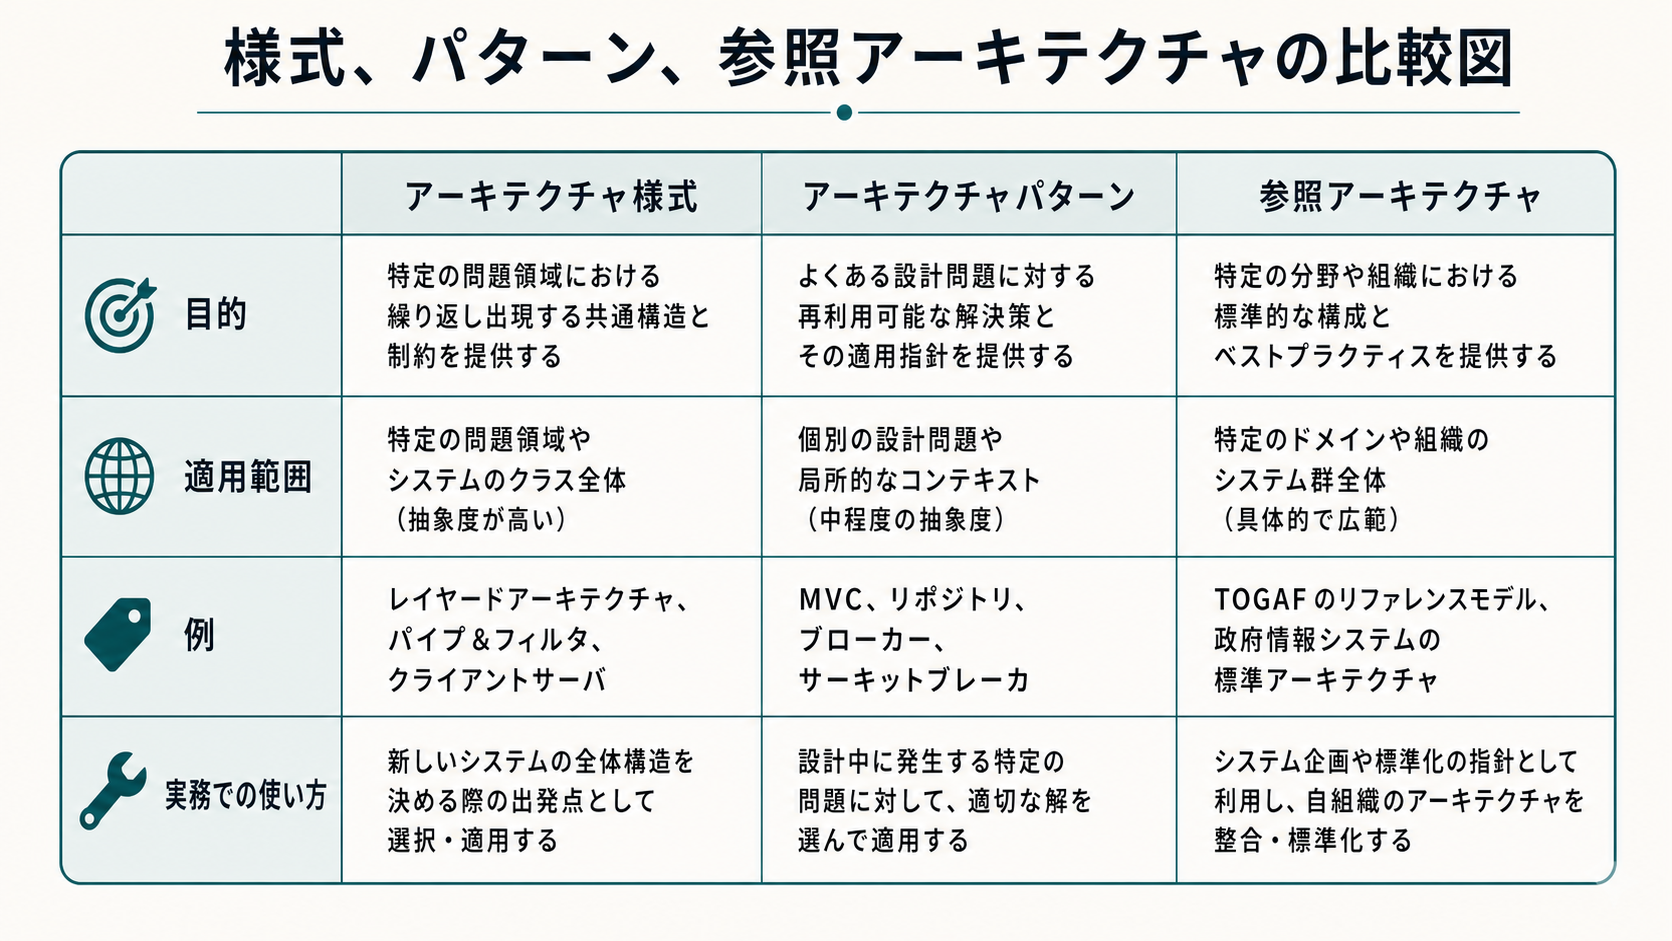
\includegraphics[width=0.96\linewidth]{swebok_structure/CH02.ソフトウェアアーキテクチャ(Software_Architecture)/2.2.ソフトウェアアーキテクチャ記述(Software_Architecture_Description)/2.2.2.アーキテクチャパターン・様式・参照アーキテクチャ(Architecture_Patterns_Styles_and_Reference_Architectures)/assets/fig-ch02-05.png}}{\fbox{\parbox[c][48mm][c]{0.9\linewidth}{\centering 画像生成待ち\\様式、パターン、参照アーキテクチャの比較図}}}
\caption{様式、パターン、参照アーキテクチャの比較図}
\label{fig:ch02-05}
\end{figure}
